% !TEX encoding = UTF-8
% !TEX TS-program = pdflatex
% !TEX root = ../tesi.tex

%**************************************************************
\chapter{Analisi dei requisiti}
\label{cap:analisi-requisiti}
%**************************************************************

Questo capitolo descrive i casi d'uso e i requisiti della piattaforma moviORDER, individuati e classificati per definire nel dettaglio obiettivi e funzionalità del sistema. I casi d'uso e i requisiti sono stati dedotti da un'analisi preliminare eseguita dal tutor aziendale, la quale è stata perfezionata dallo stagista per perseguire massima efficienza ed efficacia del sistema. Le convenzioni adottate per la stesura di casi d'uso e requisiti sono presenti in Appendice §\ref{}.

\section{Casi d'uso}

Per lo studio dei casi di utilizzo della piattaforma sono stati creati dei diagrammi dei casi d'uso che meglio descrivono funzioni e/o servizi offerti dal sistema, così come sono percepiti e utilizzati dagli attori che interagiscono con il sistema stesso. Per la definizione dei diagrammi UML dei casi d'uso è stato utilizzato lo standard UML 2.0.

\subsection{Attori del sistema}

Lo scopo di moviORDER è permettere alle aziende che forniscono dei prodotti di vendere gli stessi ai propri clienti tramite un'applicazione multipiattaforma. Quindi moviORDER viene distribuita da VISIONEIMPRESA alle aziende che forniscono prodotti, la quale viene distribuita dalle aziende stesse ai propri clienti. Gli utilizzatori finali di moviORDER sono quindi i clienti delle singole aziende che sono clienti di VISIONEIMPRESA.
L'accesso all'applicazione è consentito solamente agli utenti provvisti di credenziali di accesso, le quali vengono distribuite, insieme all'applicazione, dal fornitore. Non è prevista quindi una funzionalità di registrazione. Nel contesto di moviORDER vi sono quindi due tipologie di attori:
\begin{enumerate}
	\item \textbf{Utente non autenticato}: è un utente che non ha effettuato l'accesso al sistema al quale viene offerta la sola funzionalità di autenticazione. Una volta che un utente non autenticato viene riconosciuto accedendo al sistema, diventa un utente autenticato;
	\item \textbf{Utente autenticato}: è un utente che ha effettuato l'accesso al sistema e che può usufruire di tutte le sue funzionalità. Le funzionalità offerte all'utente autenticato sono:
	\begin{itemize}
		\item possibilità di effettuare il logout;
		\item possibilità di aggiungere articoli al proprio carrello;
		\item possibilità di modificare gli articoli nel proprio carrello;
		\item possibilità di rimuovere articoli dal proprio carrello;
		\item possibilità di inviare un ordine alla propria azienda.
	\end{itemize}
\end{enumerate}

\subsection{UC1 - Azioni utente non autenticato}

\begin{figure}[!h] 
    \centering 
    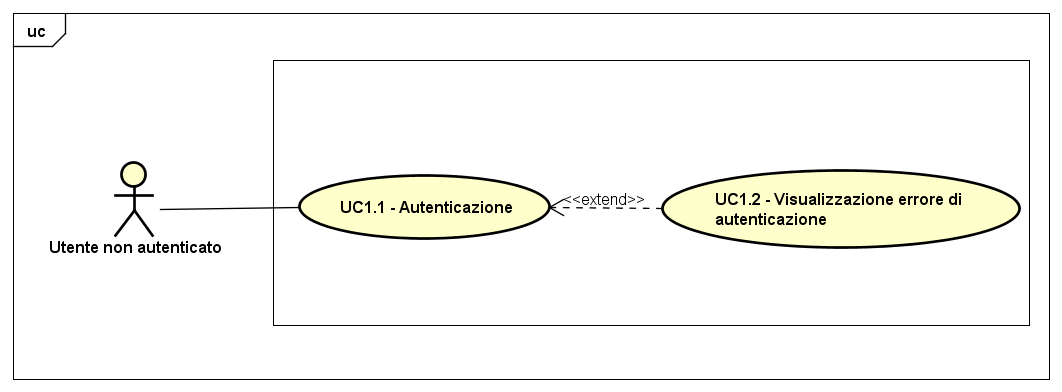
\includegraphics[width=0.9\columnwidth]{usecase/generaleNonAutenticato} 
    \caption{Use Case - UC1: Azioni utente non autenticato}
\end{figure}

\begin{itemize}
	\item \textbf{Attore}: Utente non autenticato;
	\item \textbf{Descrizione}: L'attore può eseguire l'operazione di autenticazione alla piattaforma moviORDER;
	\item \textbf{Pre-condizioni}: L'attore ha avviato l'applicazione, possiede le credenziali di accesso e non è ancora stato riconosciuto dal sistema;
	\item \textbf{Post-condizioni}: L'attore ha eseguito l'operazione di autenticazione;
	\item \textbf{Scenario principale}: UC1.1 - Autenticazione;
	\item \textbf{Scenario alternativo}: L'attore ha fornito credenziali di accesso non corrispondenti a nessun utente registrato dall'azienda, oppure non riesce ad accedere al sistema perché è stato bloccato dall'azienda stessa: UC1.2 - Visualizzazione errore di autenticazione. 
\end{itemize}

\subsection{UC1.1 - Autenticazione}

\begin{figure}[!h] 
    \centering 
    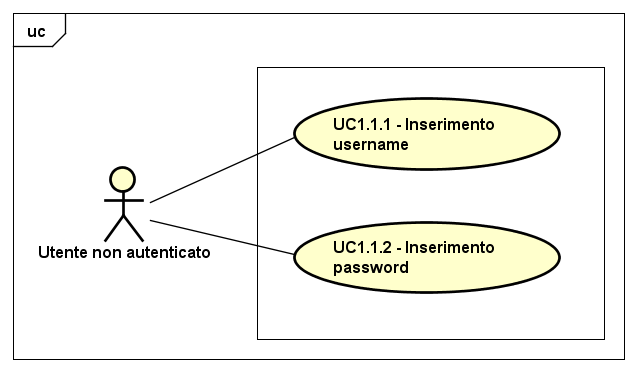
\includegraphics[width=0.9\columnwidth]{usecase/autenticazione} 
    \caption{Use Case - UC1.1: Autenticazione}
\end{figure}

\begin{itemize}
	\item \textbf{Attore}: Utente non autenticato;
	\item \textbf{Descrizione}: L'attore può eseguire l'operazione di autenticazione;
	\item \textbf{Pre-condizioni}: L’attore ha avviato l’applicazione, non è ancora riconosciuto dal sistema ed ha espresso la volontà di effettuare l’autenticazione a moviORDER;
	\item \textbf{Post-condizioni}: L’attore ha eseguito l’operazione di accesso al sistema ed è quindi ora riconosciuto come utente autenticato;
	\item \textbf{Scenario principale}: 
		\begin{enumerate}
			\item UC1.1.1 - Inserimento username;
			\item UC1.1.2 - Inserimento password.
		\end{enumerate} 
\end{itemize}

\subsection{UC2 - Azioni utente autenticato}

\begin{figure}[!h] 
    \centering 
    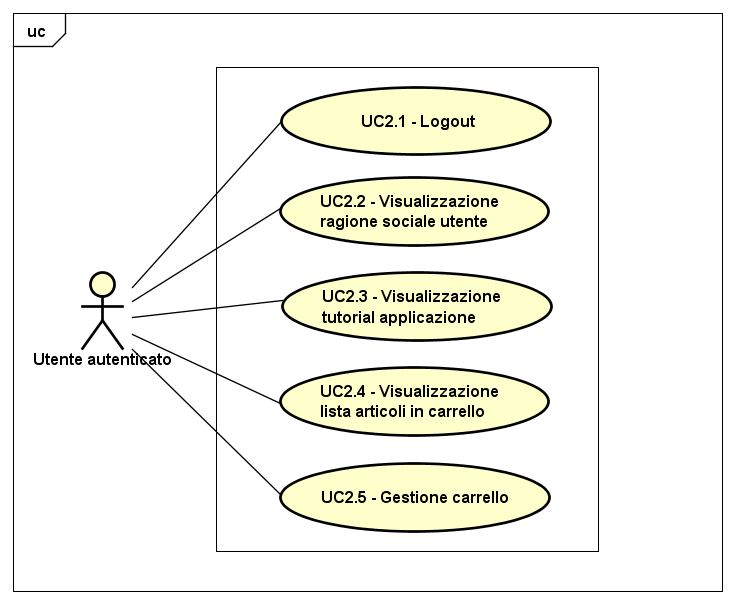
\includegraphics[width=0.9\columnwidth]{usecase/generaleAutenticato} 
    \caption{UC2 - Azioni utente autenticato}
    \label{fig:altoLivello2}
\end{figure}

\begin{itemize}
	\item \textbf{Attore}: Utente autenticato;
	\item \textbf{Descrizione}: L'attore può:
	\begin{enumerate}
		\item Eseguire l'operazione di logout;
		\item Visualizzare la propria ragione sociale;
		\item Visualizzare il tutorial dell'applicazione premendo sul relativo bottone;
		\item Visualizzare la lista degli articoli in carrello;
		\item Gestire il proprio carrello. 
	\end{enumerate}
	\item \textbf{Pre-condizioni}: L'attore è stato riconosciuto dal sistema;
	\item \textbf{Post-condizioni}: L'attore ha eseguito le azioni che desiderava compiere all'interno del sistema;
	\item \textbf{Scenario principale}: 
		\begin{enumerate}
			\item UC2.1 - Logout;
			\item UC2.2 - Visualizzazione ragione sociale utente;
			\item UC2.3 - Visualizzazione tutorial applicazione;
			\item UC2.4 - Visualizzazione lista articoli in carrello;
			\item UC2.5 - Gestione carrello.
		\end{enumerate}
\end{itemize}

\subsection{UC2.4 - Visualizzazione lista articoli in carrello}

\subsection{UC2.4.1 - Visualizzazione singolo articolo in carrello}

\subsection{UC2.5 - Gestione carrello}

\subsection{UC2.5.1 - Visualizzazione dati articolo}

\subsection{UC2.5.2 - Modifica articolo}

\subsection{UC2.5.3 - Aggiunta articolo}

\subsection{UC2.5.17 - Visualizzazione richiesta di conferma eliminazione}

\subsection{UC2.5.18 - Apertura modal di invio ordine}

\subsection{UC2.5.18.10 - Visualizzazione richiesta di conferma invio ordine}

\section{Tracciamento dei requisiti}

Da un'attenta analisi dei requisiti e degli use case effettuata sul progetto è stata stilata la tabella che traccia i requisiti in rapporto agli use case.\\
Sono stati individuati diversi tipi di requisiti e si è quindi fatto utilizzo di un codice identificativo per distinguerli.\\
Il codice dei requisiti è così strutturato R(F/Q/V)(N/D/O) dove:
\begin{enumerate}
	\item[R =] requisito
    \item[F =] funzionale
    \item[Q =] qualitativo
    \item[V =] di vincolo
    \item[N =] obbligatorio (necessario)
    \item[D =] desiderabile
    \item[Z =] opzionale
\end{enumerate}
Nelle tabelle \ref{tab:requisiti-funzionali}, \ref{tab:requisiti-qualitativi} e \ref{tab:requisiti-vincolo} sono riassunti i requisiti e il loro tracciamento con gli use case delineati in fase di analisi.

\newpage

\begin{table}%
\caption{Tabella del tracciamento dei requisti funzionali}
\label{tab:requisiti-funzionali}
\begin{tabularx}{\textwidth}{lXl}
\hline\hline
\textbf{Requisito} & \textbf{Descrizione} & \textbf{Use Case}\\
\hline
RFN-1     & L'interfaccia permette di configurare il tipo di sonde del test & UC1 \\
\hline
\end{tabularx}
\end{table}%

\begin{table}%
\caption{Tabella del tracciamento dei requisiti qualitativi}
\label{tab:requisiti-qualitativi}
\begin{tabularx}{\textwidth}{lXl}
\hline\hline
\textbf{Requisito} & \textbf{Descrizione} & \textbf{Use Case}\\
\hline
RQD-1    & Le prestazioni del simulatore hardware deve garantire la giusta esecuzione dei test e non la generazione di falsi negativi & - \\
\hline
\end{tabularx}
\end{table}%

\begin{table}%
\caption{Tabella del tracciamento dei requisiti di vincolo}
\label{tab:requisiti-vincolo}
\begin{tabularx}{\textwidth}{lXl}
\hline\hline
\textbf{Requisito} & \textbf{Descrizione} & \textbf{Use Case}\\
\hline
RVO-1    & La libreria per l'esecuzione dei test automatici deve essere riutilizzabile & - \\
\hline
\end{tabularx}
\end{table}%